% 
% Lecture Template for ME3050 -  Dynamics Modeling and Controls - Tennessee Technological University
%
% Spring 2020 - Summer 2020
% Tristan Hill, May 07, 2020
% MATLAB Review - Topic 2 - Using Simulink
%

\documentclass{beamer}                         % for presentation (has nav buttons at bottom)
%\documentclass[handout]{beamer}  % for handout 
\usepackage{beamerthemesplit}
\usepackage{amsmath}
\usepackage{listings}
\usepackage{multicol}
\usepackage{framed}

\beamertemplateballitem

% custom colors
\definecolor{TTUpurple}{rgb}{0.3098, 0.1607, 0.5176} % TTU Purple (primary)
\definecolor{TTUgold}{rgb}{1.0000, 0.8666, 0.0000} % TTU Gold (primary) 
\definecolor{mygray}{rgb}{.6, .6, .6}
\definecolor{mypurple}{rgb}{0.6,0.1961,0.8}
\definecolor{mybrown}{rgb}{0.5451,0.2706,0.0745}
\definecolor{mygreen}{rgb}{0, .39, 0}
\definecolor{mypink}{rgb}{0.9960, 0, 0.9960}

% color commands
\newcommand{\R}{\color{red}}
\newcommand{\B}{\color{blue}}
\newcommand{\BR}{\color{mybrown}}
\newcommand{\K}{\color{black}}
\newcommand{\G}{\color{mygreen}}
\newcommand{\PR}{\color{mypurple}}
\newcommand{\PN}{\color{mypink}}
\newcommand{\OR}{\color{orange}}
\newcommand{\GD}{\color{TTUgold}}

\setbeamercolor{palette primary}{bg=TTUpurple,fg=TTUgold}
\setbeamercolor{palette secondary}{bg=black,fg=TTUgold}
\setbeamercolor{palette tertiary}{bg=black,fg=TTUpurple}
\setbeamercolor{palette quaternary}{bg=TTUgold,fg=black}
\setbeamercolor{structure}{fg=TTUpurple} % itemize, enumerate, etc
\setbeamercolor{section in toc}{fg=TTUpurple} % TOC sections

%\usefonttheme{professionalfonts}

\newcommand{\Lagr}{\mathcal{L}} % lagrangian

\newcommand{\hspcu}{\underline{\hspace{20mm}}} % large horizontal space w underline
\newcommand{\vspccc}{\vspace{6mm}\\} % large vertical space
\newcommand{\vspcc}{\vspace{4mm}\\}   % medium vertical space
\newcommand{\vspc}{\vspace{2mm}\\}     % small vertical space

\newcommand{\hspcccc}{\hspace{10mm}} % large horizontal space
\newcommand{\hspccc}{\hspace{6mm}} % large horizontal space
\newcommand{\hspcc}{\hspace{4mm}}   % medium horizontal space
\newcommand{\hspc}{\hspace{2mm}}     % small horizontal space

\newcommand{\eqscl}{0.9}     % small horizontal space


\author{ME3060 - Dynamics Modeling and Controls Lab} % original formatting from Mike Renfro, September 21, 2004

\newcommand{\MNUM}{1\hspace{2mm}} % Module number
\newcommand{\TNUM}{2\hspace{2mm}} % Topic number 
\newcommand{\moduletitle}{MATLAB Review }
\newcommand{\topictitle}{Using Simulink} 

\newcommand{\sectiontitleI}{What is Simulink?}
\newcommand{\sectiontitleII}{Create a Model}
\newcommand{\sectiontitleIII}{Run the Model}
\newcommand{\sectiontitleIV}{View and Export Results}

% custom box
\newsavebox{\mybox}

\title{Demonstration \MNUM - \moduletitle}

\date{Mechanical Engineering\vspc Tennessee Technological University}

\begin{document}

\lstset{language=MATLAB,basicstyle=\ttfamily\small,showstringspaces=false}

\frame{\titlepage \center\begin{framed}\Large \textbf{Topic \TNUM - \topictitle}\end{framed} \vspace{5mm}}

% Section 0: Outline
\frame{

\large \textbf{Topic \TNUM - \topictitle} \vspace{3mm}\\

\begin{multicols}{2}
\begin{itemize}

	\item \sectiontitleI		\vspc % Section I
	\item \sectiontitleII 	\vspc % Section II
	\item \sectiontitleIII 	\vspc %Section III
	\item \sectiontitleIV 	\vspc %Section IV

\end{itemize}

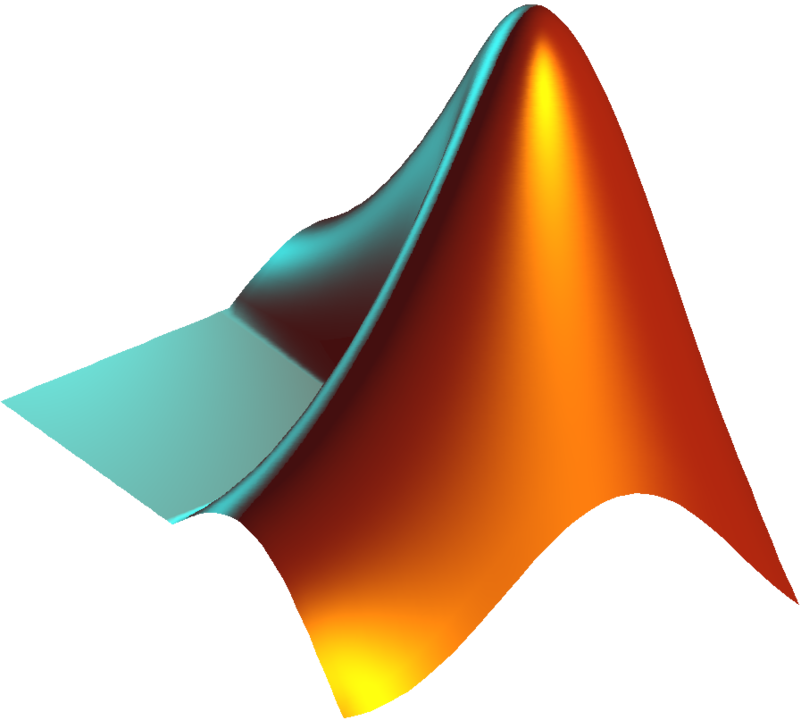
\includegraphics[scale=.2]{matlab_logo.png}
\end{multicols}
}

% Section I:
\section{\sectiontitleI}

% Section I - Frame I:
\frame{
\frametitle{\sectiontitleI}

Simulink is a MATLAB-based {\PR graphical programming} environment for {\B modeling}, {\B simulating} and {\B analyzing} multidomain dynamical systems. Its primary interface is a graphical {\OR block diagramming} tool and a customizable set of block libraries. It offers tight integration with the rest of the MATLAB {\R environment} and can either {\PN drive} MATLAB or be {\PN scripted} from it. Simulink is widely used in {\G automatic control} and digital {\G signal processing} for multidomain simulation and model-based design.[2][3] 

\vspace{5mm}
{\tiny Text: \href{https://en.wikipedia.org/wiki/Simulink}{Wikipedia} } 
}


% Section II:
\section{\sectiontitleII}

% Section II - Frame I:
\frame{
\frametitle{\sectiontitleII}
 
\begin{itemize}

\item While {\PR installing} MATLAB you can choose to include simulink. If you did not can can {\PN install} it through the {\it Add-Ons Explorer} in the home tab. \vspc

\item Open MATLAB and {\G start simulink} by entering the following in to the command window. \vspc

\scalebox{1.0}{{\fontfamily{qcr}\selectfont  \hspace{5mm} >>  simulink}} \vspc

\item {\R Wait} for Simulink to open, and then click {\B blank model}. \vspc $\rightarrow$ A simulink file is called a {\it model}\hspc (.slx) 

\end{itemize}

}

% Section II - Frame II:
\frame{
\frametitle{\sectiontitleII}

You begin with a blank model (as you selected) and the possibilities are endless. Alternatively you could start with a {\BR template}.  \vspc

Click on  the {\OR Library Browser} to find components to add  to the model. \vspc


\vspace{30mm}

}




% Section III:
\section{\sectiontitleIII}

\frame{
\frametitle{\sectiontitleIII}


}

% Section IV:
\section{\sectiontitleIV}

\frame{
\frametitle{\sectiontitleIV}

}
	
\end{document}





